%====================================================================
\subsection{Statistical inference: frequentist / Bayesian}
\frame{\frametitle{Outline} \tableofcontents[currentsubsection]}
%====================================================================
\frame{ \frametitle{An example}

  \paragraph{Example:} 
  \begin{itemize}
   \item $n$ tissue samples: $i = 1 \dots n$
   \item $Y_i =$ status (0 = n, normal = tumor) of sample $i$ 
   \item $\xbf_i = (x_{i1}, \dots x_{ip}) =$ vector of gene expression for sample $i$ (gene $j = 1 \dots p$)
  \end{itemize}
  
  \bigskip \bigskip 
  \paragraph{Dataset:} $n = 78$, $p=15$
  \begin{center} {\tt \begin{tabular}{lrrrcr}
  & AB033066  & NM003056  & NM000903  & \dots & Status \\ 
  \hline 
  1  & 0.178  & 0.116  & 0.22  & & 0 \\ 
  2  & 0.065  & -0.073  & -0.014  & & 0 \\ 
  3  & -0.077  & 0.03  & 0.043  & & 0 \\ 
  4  & 0.176  & -0.041  & 0.362  & & 0 \\ 
  5  & -0.089  & -0.164  & -0.266  & & 0 \\
  & \multicolumn{4}{c}{$\underbrace{\qquad\qquad\qquad\qquad\qquad}$} & \multicolumn{1}{r}{$\underbrace{\quad}$} \\
  & \multicolumn{4}{c}{$X$} & \multicolumn{1}{r}{$Y\;\;$}
  \end{tabular} } \end{center}
  
  \pause \bigskip 
  Similar question for genotyping data: $x_{ij} \in \{0, 1, 2\}$.
  }
  
%====================================================================
\frame{ \frametitle{A statistical model}

  \paragraph{Model:} Logistic regression
  \begin{itemize}
   \item The samples are independent.
   \item The probability for sample $i$ to be tumor depends on $\xbf_i$:
   $$
   \Pr\{Y_i = 1\} = \frac{e^{\xbf_i^\intercal \thetabf}}{1 + e^{\xbf_i^\intercal \thetabf}}, 
   \qquad \qquad
   \xbf_i^\intercal \thetabf = \sum_{j=1}^p x_{ij} \theta_j
   $$
   \item $\thetabf = (\theta_1, \dots \theta_p):$ unknown parameter (regression coefficients, incl. intercept)
  \end{itemize}
  
  $$
  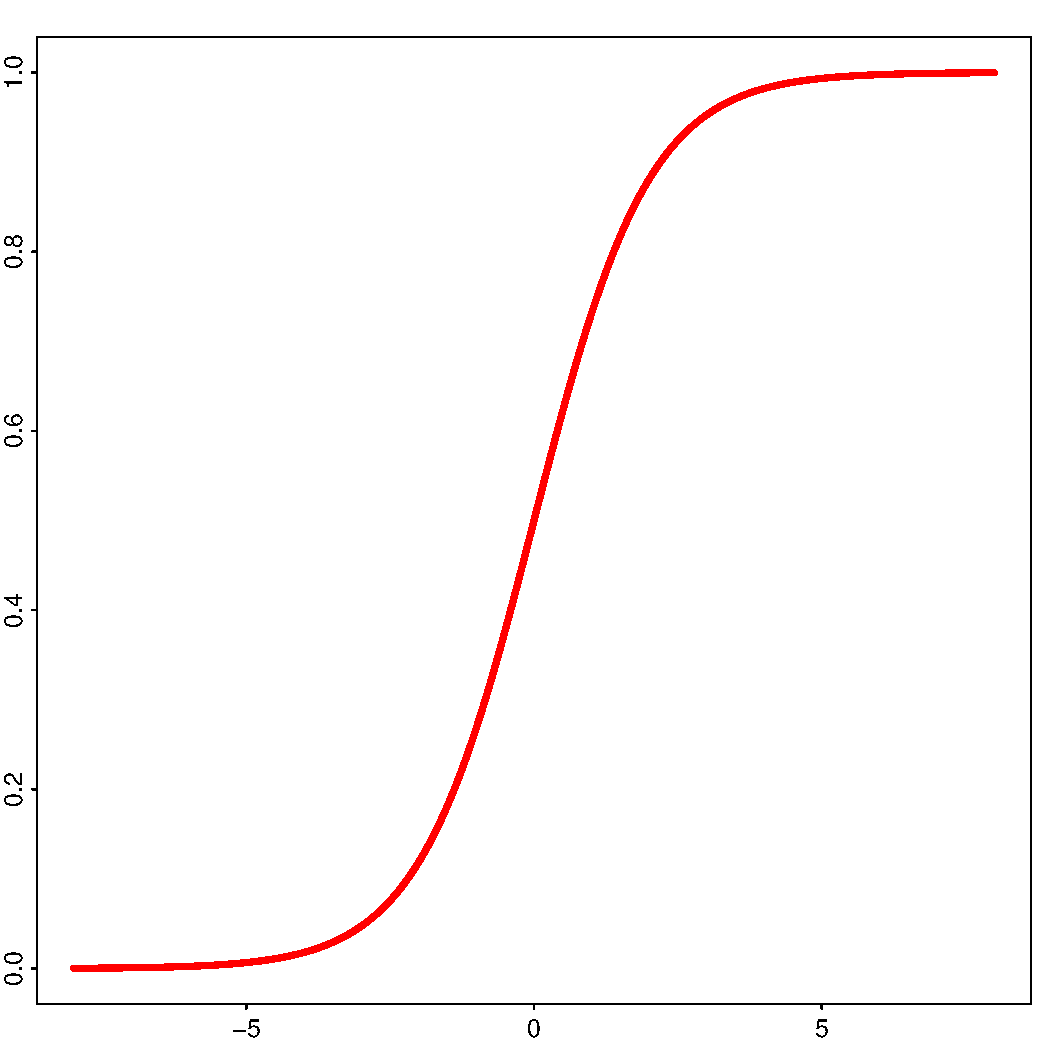
\includegraphics[width=.6\textwidth, height=.4\textheight]{\figfig/logistic-curve}
  $$
}  

%====================================================================
\frame{ \frametitle{Frequentist inference}

  \paragraph{$\thetabf =$ fixed parameter:}
  \begin{itemize}
   \item Statistical model:
   $$
   \Ybf \sim p_\thetabf
   $$
   \item Inference: get a (point) estimate $\widehat{\thetabf}$ e.g.
   $$
   \widehat{\thetabf}: \qquad \log p_{\widehat{\thetabf}}(\Ybf) = \max_\thetabf \log p_{\thetabf}(\Ybf)
   $$
   \item The estimate $\widehat{\thetabf}$ itself is random (depends on the data) \ra conf. interval, tests, ...
  \end{itemize}
  
  \bigskip \bigskip \pause
  \paragraph{Output:} {\tt GLM = glm(Y $\sim$ X, family=binomial)}
  \begin{center} {\tt \begin{tabular}{lrrrr}
    & Estimate  & Std. Error  & z value  & Pr($>|$z$|$) \\ 
    \hline 
    (Intercept)  & -0.7212697  & 0.6512707  & -1.107481  & 0.2680861 \\ 
    XAB033066  & 7.23375  & 2.505118  & 2.887589  & 0.003882068 \\ 
    XNM003056  & -0.6116423  & 1.854695  & -0.3297806  & 0.7415658 \\ 
    XNM000903  & 1.732625  & 1.199888  & 1.443988  & 0.1487423 \\
    \dots
    \end{tabular} } \end{center}
}

%====================================================================
\frame{ \frametitle{Bayesian inference}

  \paragraph{$\thetabf =$ random parameter:}
  \begin{itemize}
   \item Statistical model:
   $$
   \emphase{\ell(\Ybf \gv \thetabf)} := p(\Ybf \gv \thetabf) \qquad \text{($=$ {\sl likelihood})}
   $$
   \item Inference: provide the conditional distribution of $\thetabf$ given the observed data $\Ybf$:
   $$
   p(\thetabf \gv \Ybf) \qquad \text{($=$ {\sl posterior} distribution)}
   $$
   \ra credibility intervals
   \item Requires to define a marginal distribution: 
   $$
   \emphase{\pi(\thetabf)} := p(\thetabf) \qquad \text{($=$ {\sl prior} distribution)}
   $$  
  \end{itemize}
}

%====================================================================
\subsection{Basics of Bayes inference}
\frame{\frametitle{Outline} \tableofcontents[currentsubsection]}
%====================================================================
\frame{ \frametitle{Why 'Bayes'}

  \paragraph{Bayes formula:}
  $$
  P(A \gv B) = \frac{P(A, B)}{P(B)} = \frac{P(A)}{P(B)} P(B \gv A)
  $$
  \begin{itemize}
   \item $P(B) =$ marginal probability of $B$
   \item $P(A, B) =$ joint probability of $A$ and $B$
   \item $P(A \gv B) =$ conditional probability of $A$ given $B$ 
  \end{itemize}

  \bigskip \bigskip \pause
  \paragraph{Be careful.} Many methods, e.g.
  $$
  \text{Bayesian network, Naive Bayes, ...}
  $$
  \begin{itemize}
  \item use conditional probabilities
  \item but have nothing to do with Bayesian inference (in the statistical sense)
  \end{itemize}
}

%====================================================================
\frame{ \frametitle{Bayes formula for Bayesian inference (1/2)}

  \paragraph{Posterior distribution.}
  $$
  p(\thetabf \gv \Ybf) = \frac{p(\Ybf, \thetabf)}{p(\Ybf)} = \frac{\overset{prior}{\overbrace{\pi(\thetabf)}} \; \overset{likelihood}{\overbrace{\ell(\Ybf \gv \thetabf)}}}{\emphase{p(\Ybf)}}
  $$
  \ra Requires to evaluate the {\sl integrated likelihood} (i.e. marginal)
  $$
  p(\Ybf) = \int \pi(\thetabf) \ell(\Ybf \gv \thetabf) \d \thetabf,
  $$
  which acts as the normalizing constant of the posterior $p(\thetabf \gv \Ybf)$.
}

%====================================================================
\frame{ \frametitle{Bayes formula for Bayesian inference (2/2)}

  \paragraph{Remarks.}
  \begin{enumerate}
   \item \pause Computing $p(\Ybf)$ is generally (very) difficult: see Section \ref{sec:MCMC} \\~
   \item \pause Obviously
   $$
   p(\thetabf \gv \Ybf) \propto \pi(\thetabf) \; \ell(\Ybf \gv \thetabf),
   $$
   \ra $p(\thetabf \gv \Ybf)$ and $p(\thetabf' \gv \Ybf)$ can be compared, \emphase{without computing $p(\Ybf)$} \\~
   \item \pause Obviously, the posterior $p(\thetabf \gv \Ybf)$ depends on the prior $\pi(\thetabf)$ (see next slides) \\ ~
   \item \pause $p(\cdot)$ is sometimes denoted $[\cdot]$:
   $$
   p(\thetabf \gv \Ybf) = \frac{\pi(\thetabf) \; \ell(\Ybf \gv \thetabf)}{p(\Ybf)}
   \qquad \Leftrightarrow \qquad
   [\thetabf \gv \Ybf] = \frac{[\thetabf] \; [\Ybf \gv \thetabf]}{[\Ybf]}
   $$ 
  \end{enumerate}

}
%====================================================================
\frame{ \frametitle{The posterior depends on the prior} \label{slide:prior}

  \begin{tabular}{cc}
    \begin{tabular}{p{.5\textwidth}}
    \paragraph{Data \& Model:}
    \begin{itemize}
     \item $Y_i =1$ if disease, $0$ otherwise
     \item $n = 10$ patients
     \item $\vdots:$ number disease carriers$/ n$
    \end{itemize}

    \bigskip \pause
    \paragraph{Param:}
    \begin{itemize}
     \item $\theta =$ proba. disease
     \item $\textcolor{blue}{\boldsymbol{-}}:$ prior $\pi(\theta)$
    \end{itemize}

    \bigskip \pause
    \paragraph{Output:}
    \begin{itemize}
     \item $\boldsymbol{-}:$  posterior $p(\theta \gv \Ybf)$
    \end{itemize}

    \end{tabular}
    & 
    \hspace{-.02\textwidth}
    \begin{tabular}{p{.5\textwidth}}
	 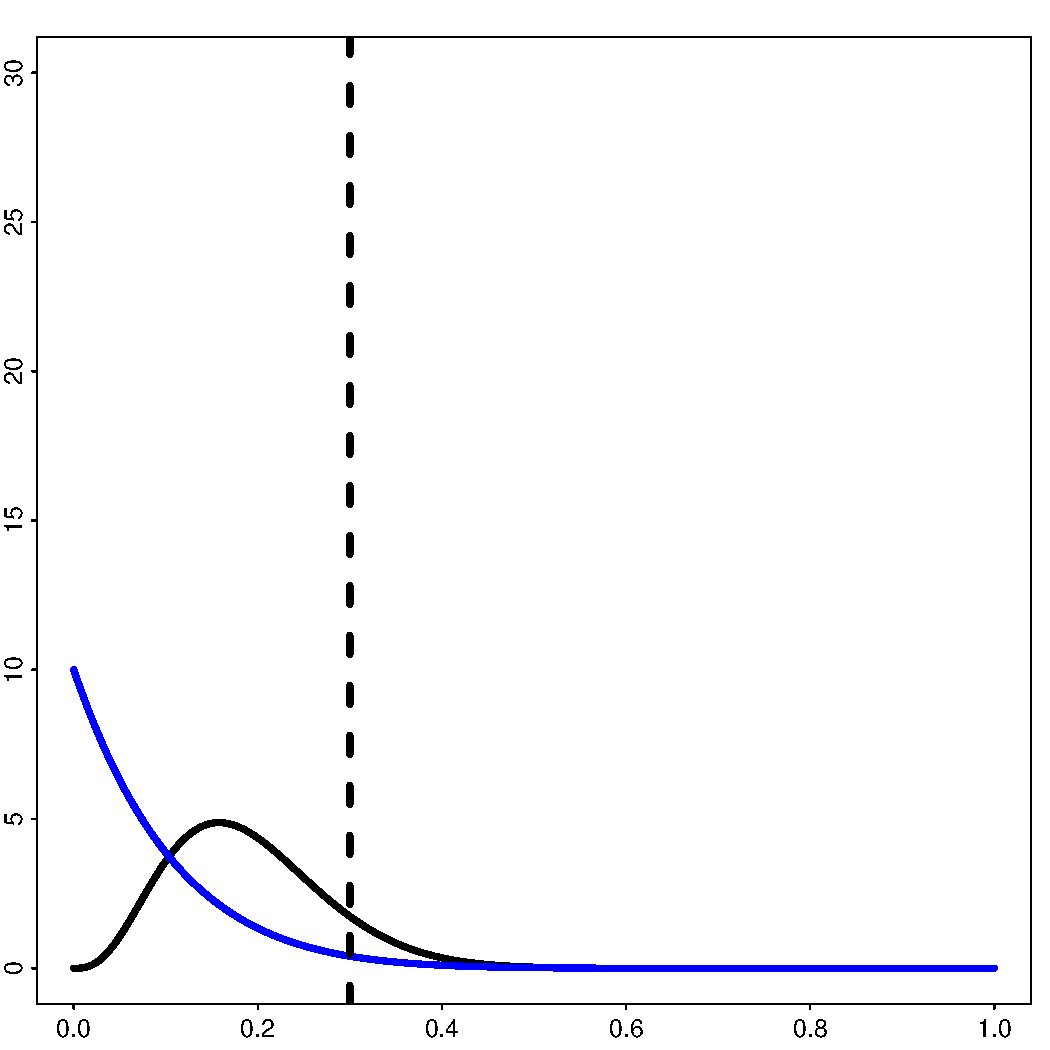
\includegraphics[width=.3\textwidth, height=.3\textheight]{../figs/beta-binomial-a1-b10-n10-p33} \\
	 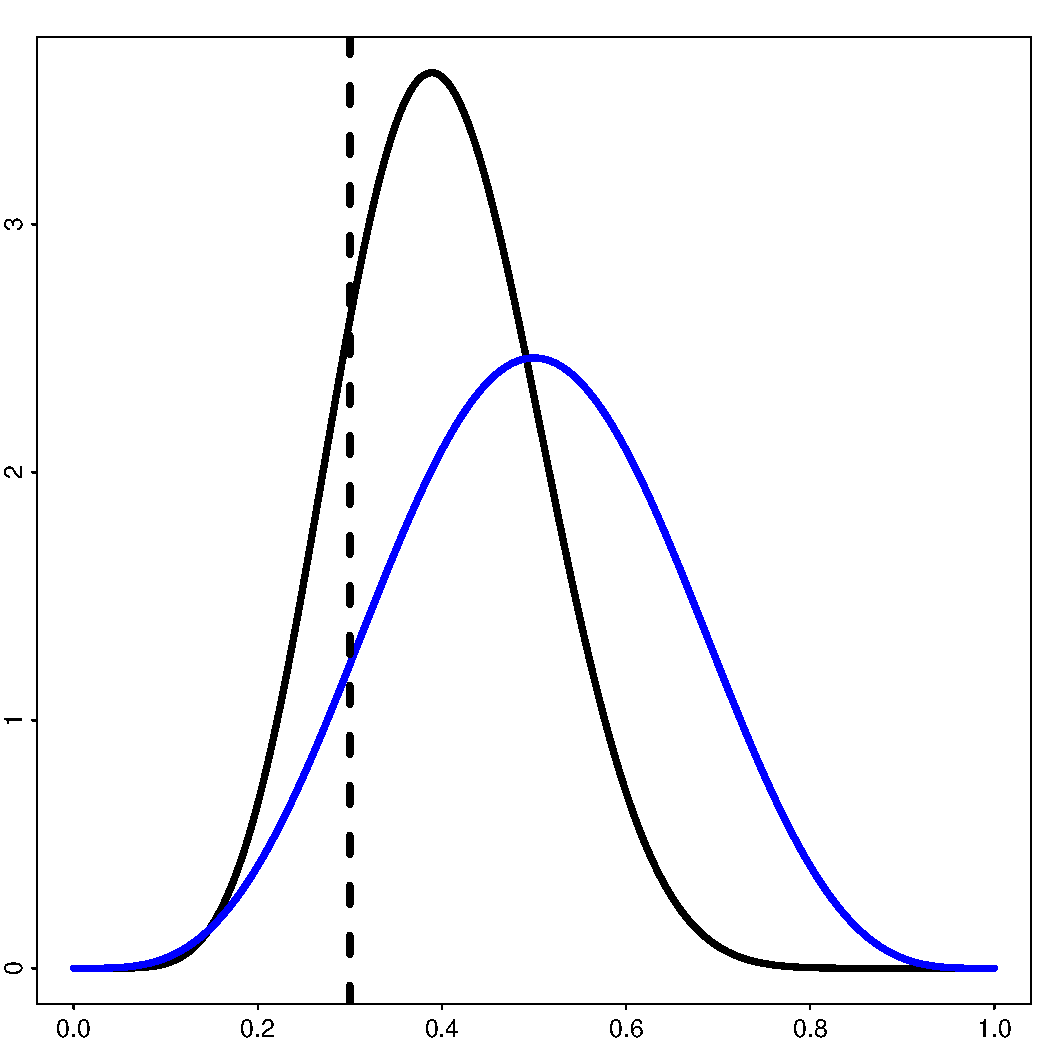
\includegraphics[width=.3\textwidth, height=.3\textheight]{../figs/beta-binomial-a5-b5-n10-p33} \\
	 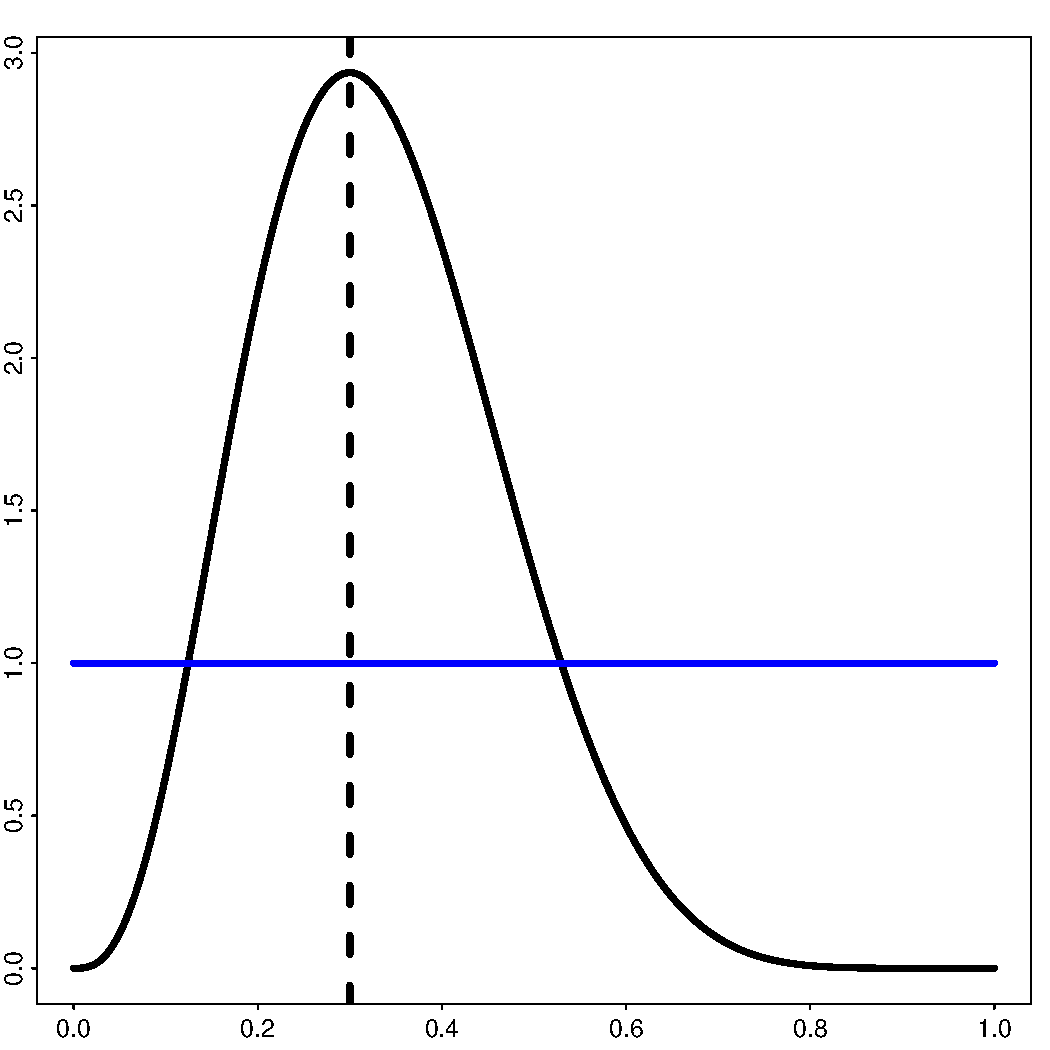
\includegraphics[width=.3\textwidth, height=.3\textheight]{../figs/beta-binomial-a1-b1-n10-p33} 
    \end{tabular}
  \end{tabular}
}

%====================================================================
\frame{ \frametitle{Dependency vanishes when $n$ increases}

  \begin{tabular}{ccc}
    $n = 10$ & $n = 100$ & $n = 1000$ \\
	 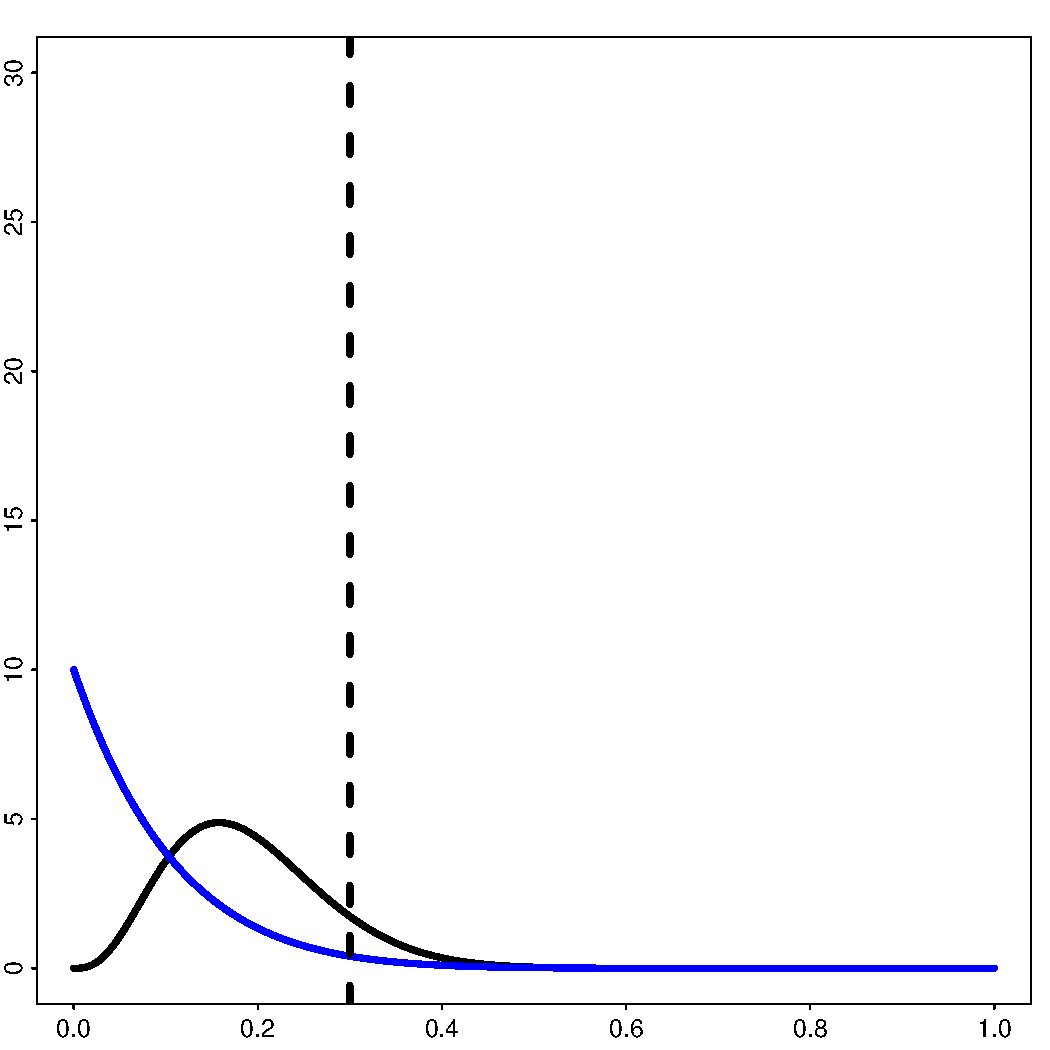
\includegraphics[width=.3\textwidth, height=.25\textheight]{../figs/beta-binomial-a1-b10-n10-p33} & 
	 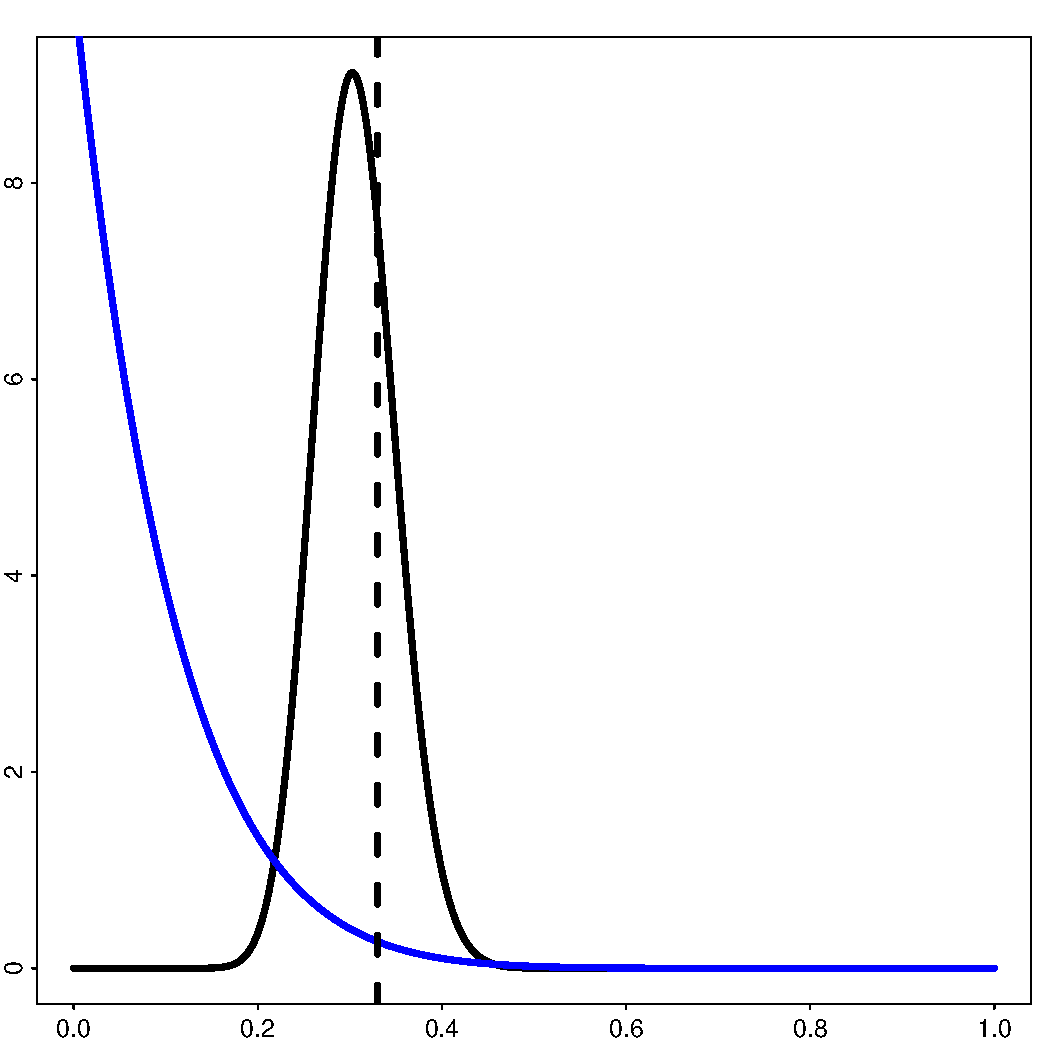
\includegraphics[width=.3\textwidth, height=.25\textheight]{../figs/beta-binomial-a1-b10-n100-p33} & 
	 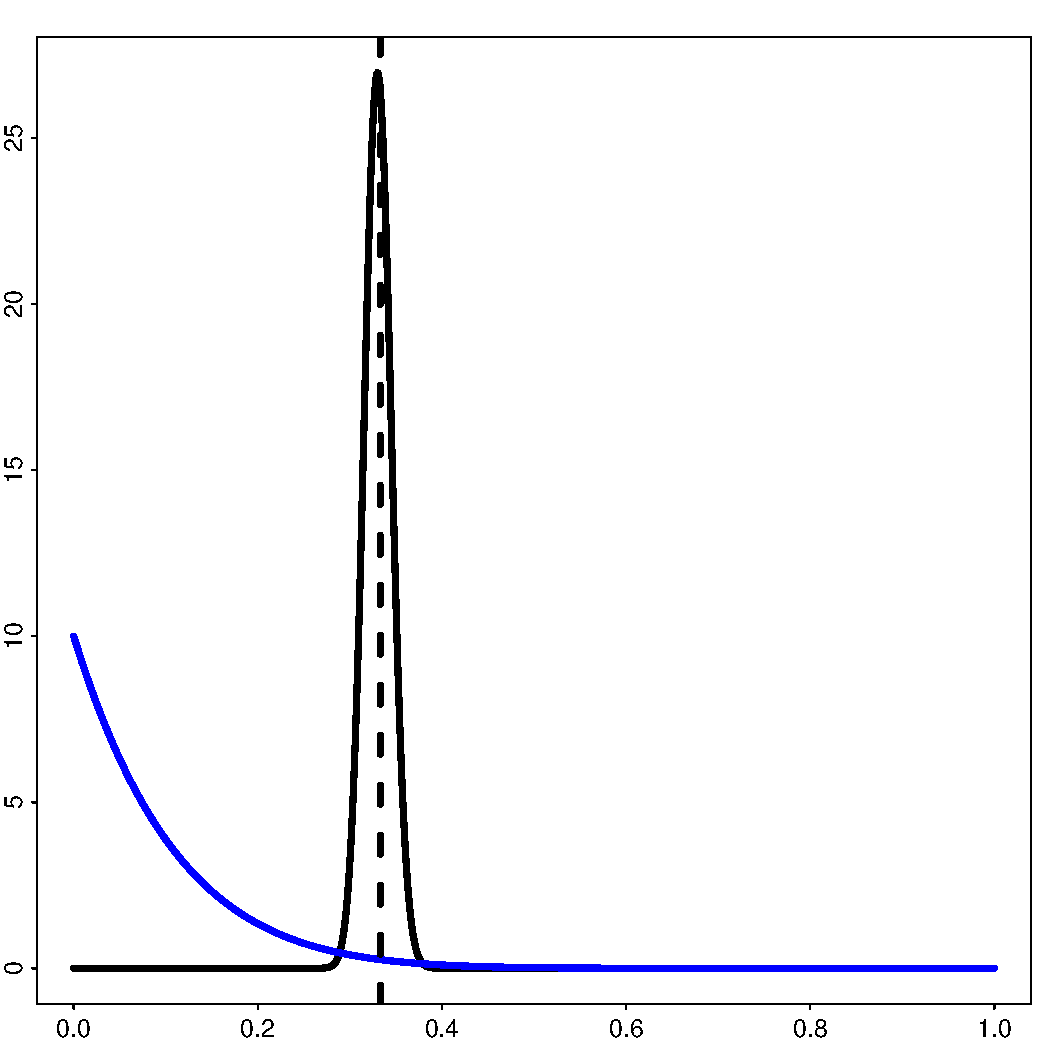
\includegraphics[width=.3\textwidth, height=.25\textheight]{../figs/beta-binomial-a1-b10-n1000-p33} 
	 \\
	 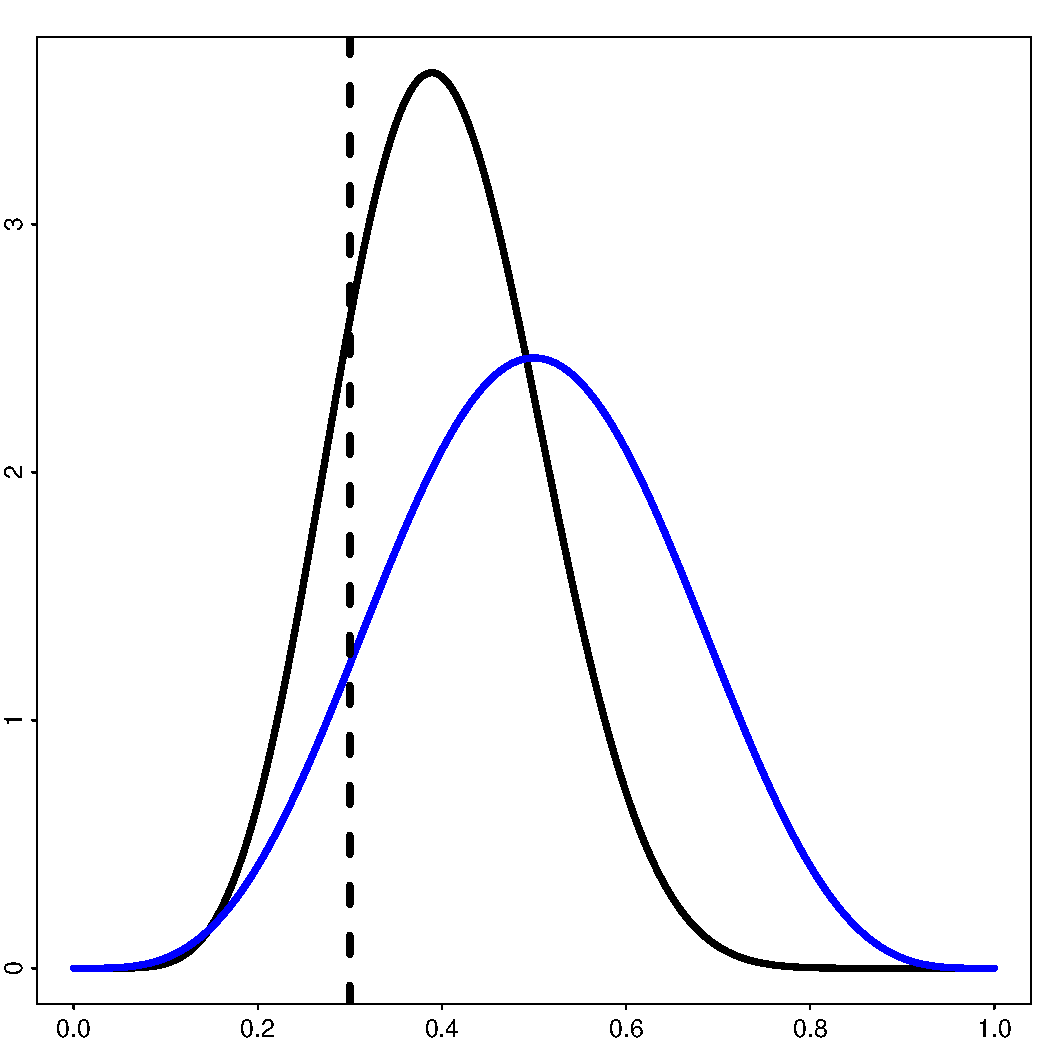
\includegraphics[width=.3\textwidth, height=.25\textheight]{../figs/beta-binomial-a5-b5-n10-p33} & 
	 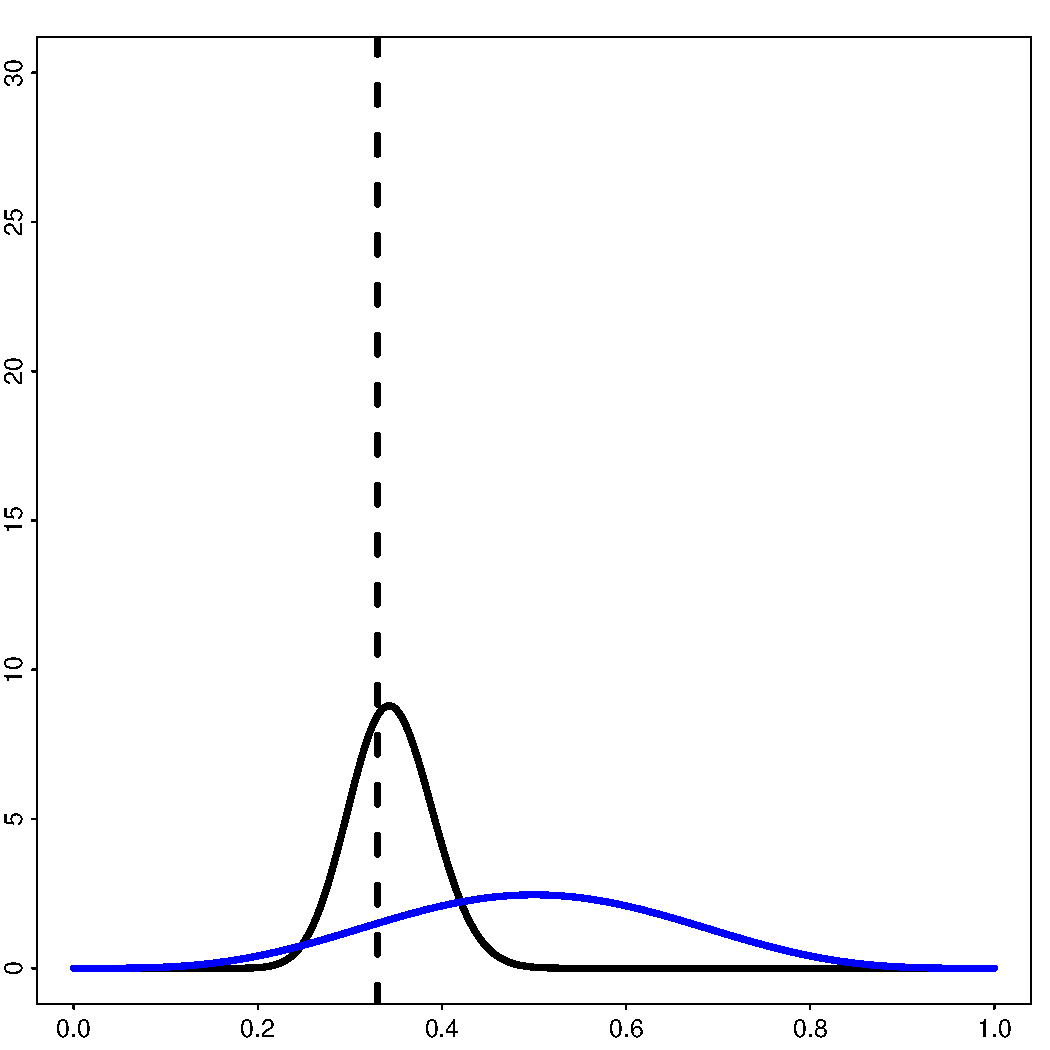
\includegraphics[width=.3\textwidth, height=.25\textheight]{../figs/beta-binomial-a5-b5-n100-p33} & 
	 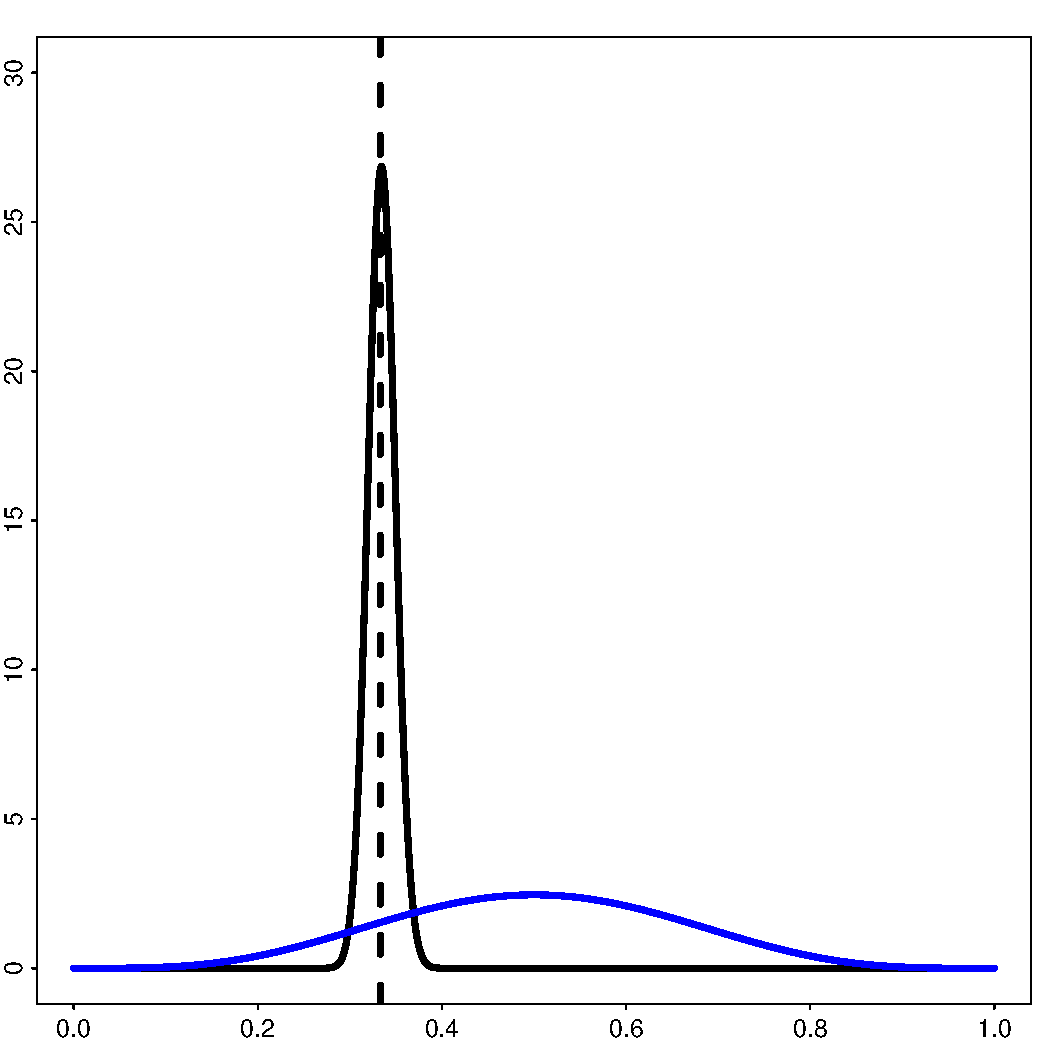
\includegraphics[width=.3\textwidth, height=.25\textheight]{../figs/beta-binomial-a5-b5-n1000-p33} 
	 \\
	 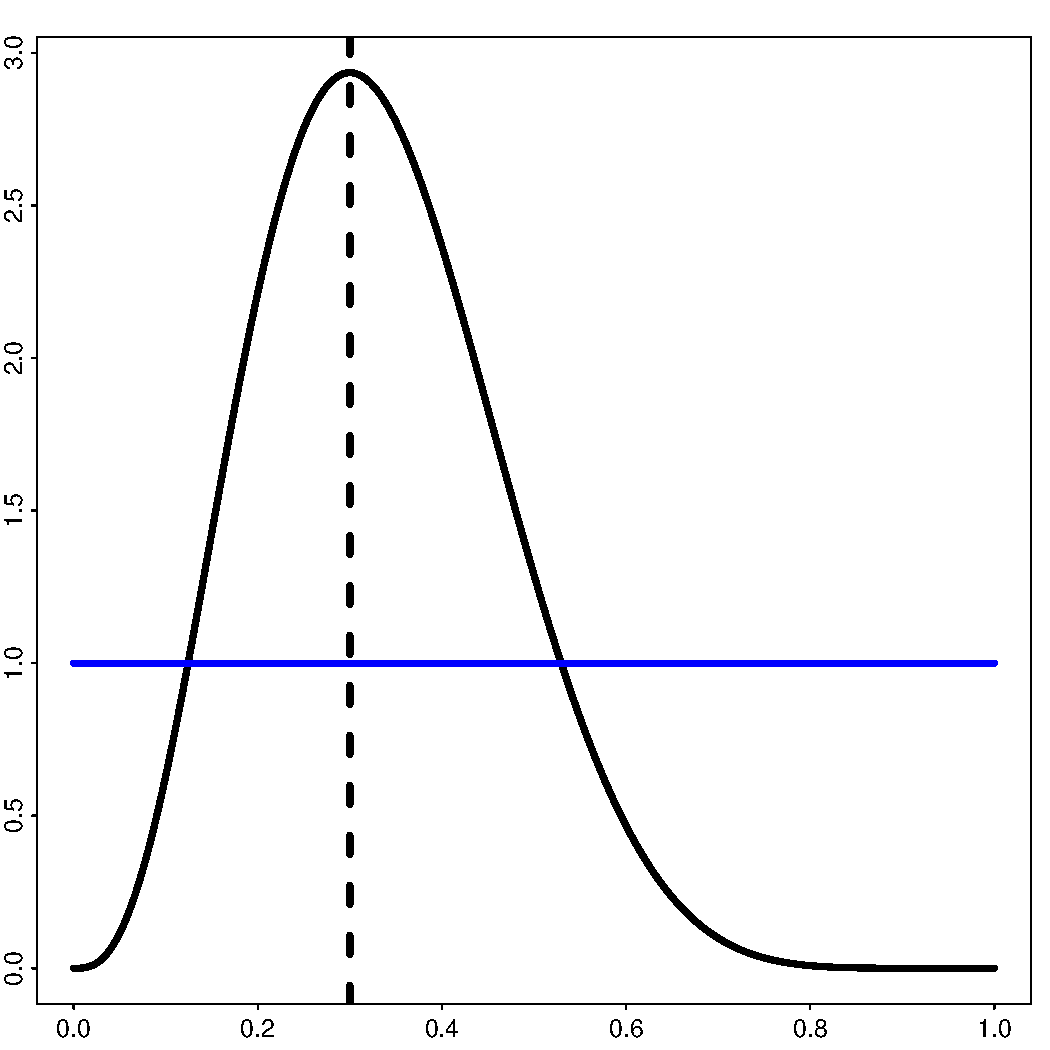
\includegraphics[width=.3\textwidth, height=.25\textheight]{../figs/beta-binomial-a1-b1-n10-p33} & 
	 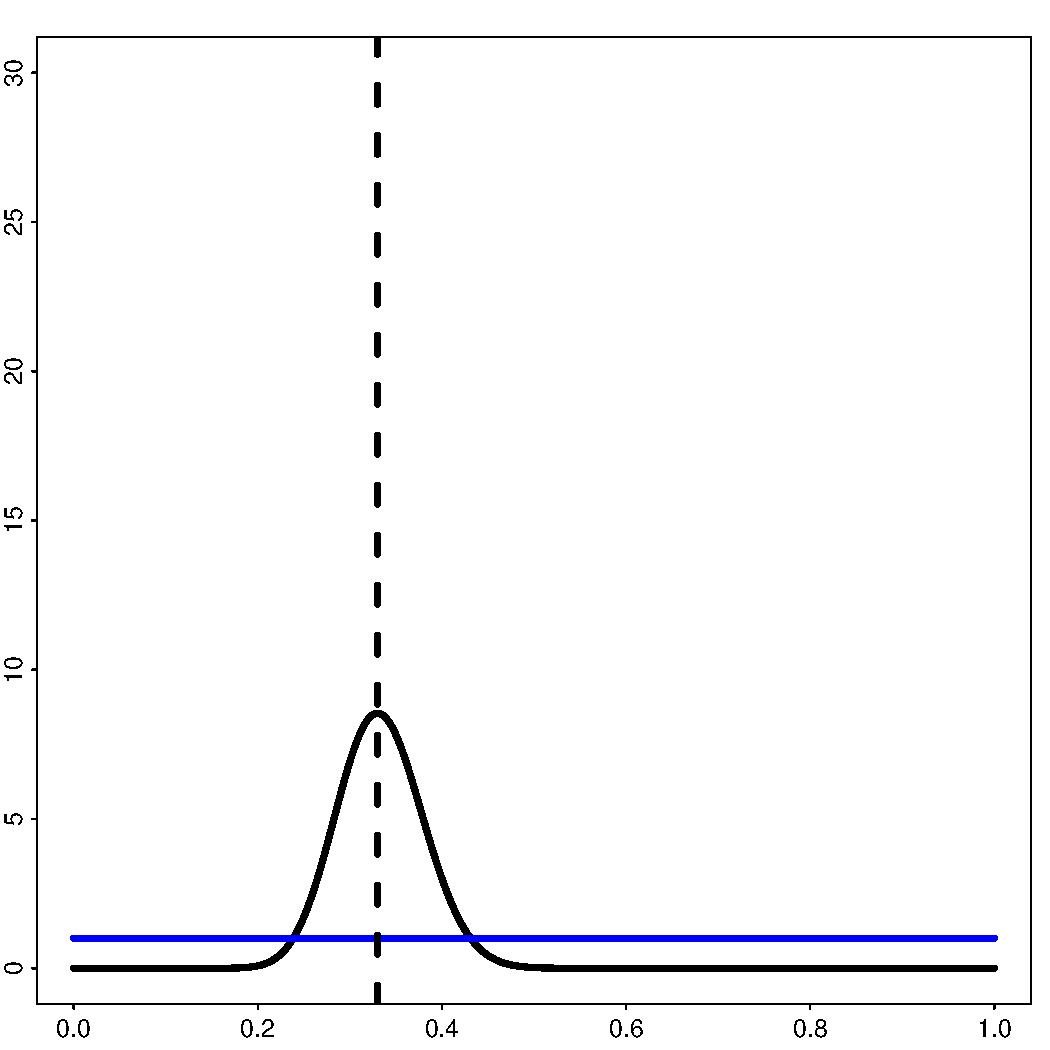
\includegraphics[width=.3\textwidth, height=.25\textheight]{../figs/beta-binomial-a1-b1-n100-p33} & 
	 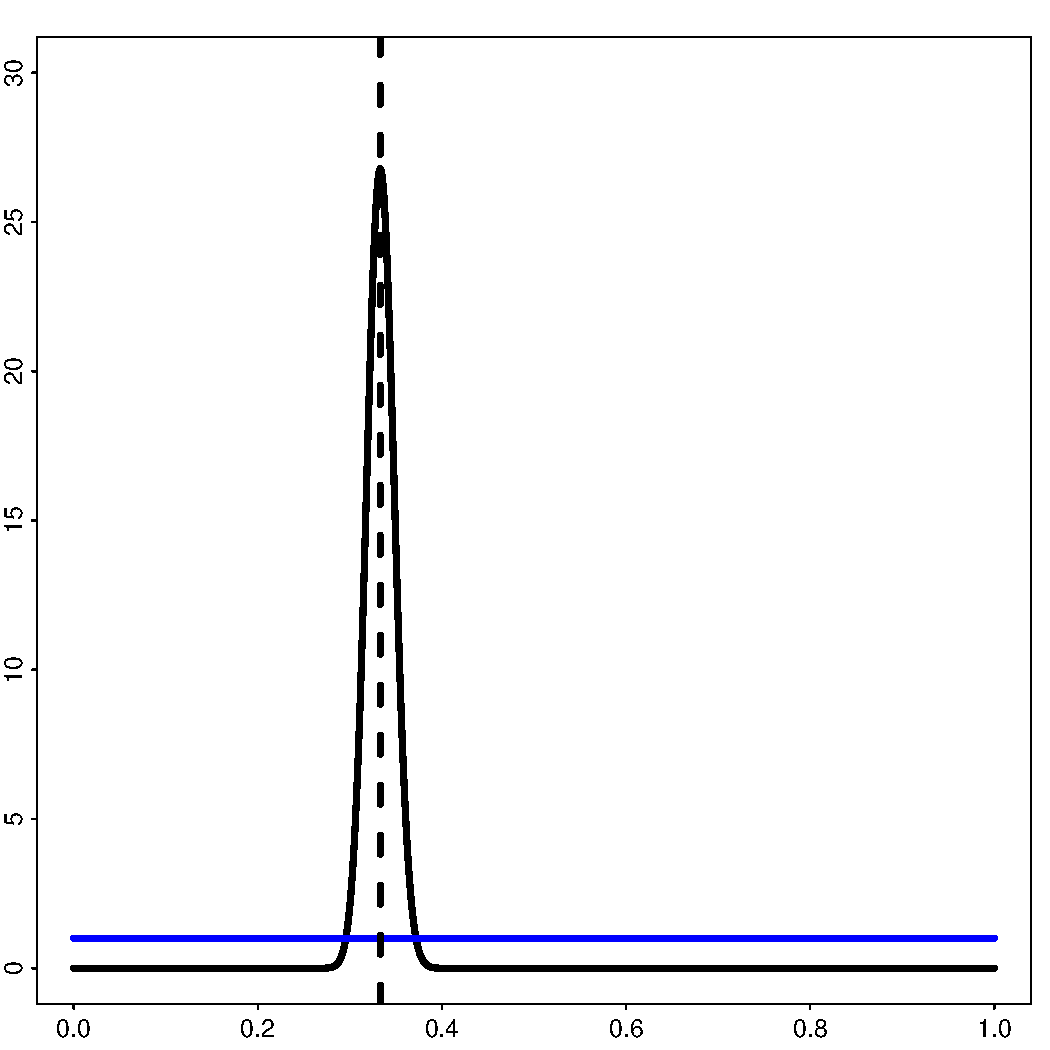
\includegraphics[width=.3\textwidth, height=.25\textheight]{../figs/beta-binomial-a1-b1-n1000-p33} 
  \end{tabular}
}

%====================================================================
\frame{ \frametitle{Back to logistic regression}

  \paragraph{Model}
  \begin{itemize}
   \item Prior: coefficients $\theta_j$ all independent:
   $$
   \theta_j \sim \Ncal(0, 100)
   $$
   \item Likelihood: all samples independent, {\sl conditionally} on $\thetabf$:
   $$
   \Pr\{Y_i = 1 \gv \thetabf\} = e^{\xbf_i^\intercal \thetabf} \left/ \left( 1 + e^{\xbf_i^\intercal \thetabf} \right) \right. 
   $$
  \end{itemize}
  
  \bigskip \pause
  \paragraph{Inference:}
  $$
  \thetabf \gv \Ybf \sim \; ? 
  $$
  (for sure: $p(\thetabf \gv \Ybf) \neq \Ncal(\cdot, \cdot)$).
}

%====================================================================
\frame{ \frametitle{Bayesian inference}

  \paragraph{Output:} 
  $$
  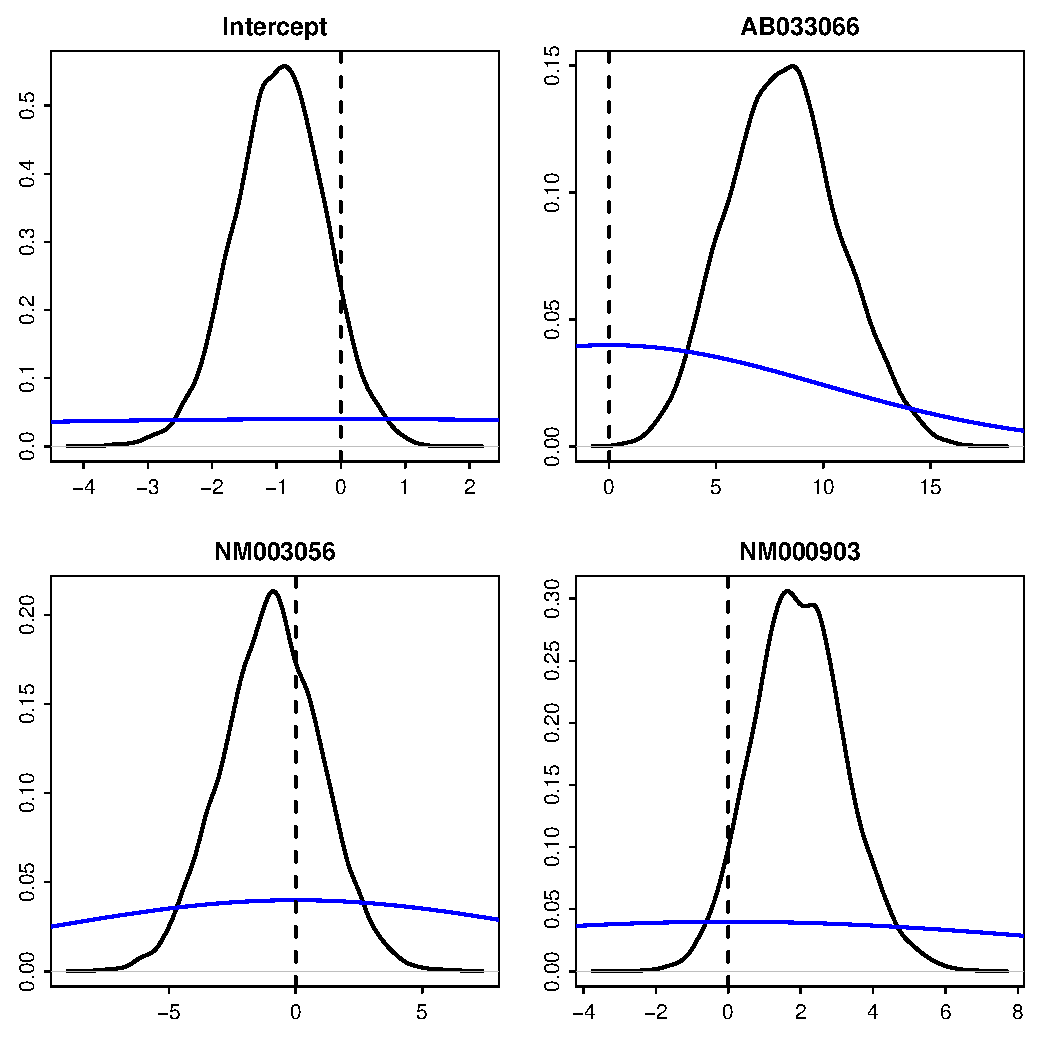
\includegraphics[width=.8\textwidth, height=.8\textheight]{\figfig/posterior-density}
  $$
}

%====================================================================
\frame{ \frametitle{No test (and no estimator)} 

  \paragraph{Frequentist hypothesis:}
  $$
  H_0 = \{\theta = 0\}
  $$
  \ra meaningless when $\theta$ is random: $P(H_0 \gv \Ybf) = 0$
  
  \pause \bigskip \bigskip
  \paragraph{Bayesian assessment:}
  $$
  CI_{1 - \alpha}(\theta \gv \Ybf) \ni 0 \; ?
  $$

  \pause \bigskip \bigskip
  \paragraph{Parameter estimate.} For the same reason:
  $$
  \widehat{\theta} \text{ can no be an estimate of } \theta
  $$
  (because $\theta$ is random).
  
}

%====================================================================
\subsection{Some typical uses of Bayesian inference}
\frame{\frametitle{Outline} \tableofcontents[currentsubsection]}
%====================================================================
\frame{ \frametitle{Posterior distribution and confidence intervals} \label{sec:CI}

  \paragraph{Parameter 'estimate'.}
  \begin{align*}
   \text{posterior mean:} \qquad \widehat{\theta}_j & = \Esp(\theta_j \gv \Ybf)  \\
   \text{posterior mode:} \qquad \widehat{\theta}_j & = \arg\max _{\theta_j} \; p(\theta_j \gv \Ybf)
  \end{align*}

  \bigskip
  \paragraph{Credibility interval (CI).} With level $1 - \alpha$ (e.g. 95\%):
  $$
  CI_{1-\alpha}(\theta_j \gv \Ybf) = [\theta_j^\ell; \theta_j^u]:
  \qquad 
  \Pr\{\theta_j^\ell < \theta_j < \theta_j^u \gv \Ybf\} = 1-\alpha
  $$

  \bigskip \pause
  \paragraph{Example.} \appref{app:CIcontrast}
  \begin{center} {\tt \begin{tabular}{lrrrcr}
  & post.mean  & post.mode  & lower.CI  & upper.CI \\ 
  \hline 
  Intercept  & -0.890718  & -0.9281564  & -2.266244  & 0.4477921 \\ 
  AB033066  & 8.483059  & 8.229936  & 3.595861  & 13.60357 \\ 
  NM003056  & -0.8067056  & -1.290723  & -4.698653  & 3.000588 \\ 
  NM000903  & 2.13275  & 1.958102  & -0.3106497  & 4.750834     
  \end{tabular} } \end{center}
}

%====================================================================
\frame{ \frametitle{Accounting for uncertainty}

  \paragraph{Question:} What is the probability for sample 0 (with profile $\xbf_0$) to be tumor?

  \bigskip \bigskip 
  \paragraph{Model answer:}
  $$
  \Pr\{Y_0 = 1 \gv \thetabf\} = e^{\xbf_0^\intercal \thetabf} \left/ \left( 1 + e^{\xbf_0^\intercal \thetabf} \right) \right. 
  $$
  but $\thetabf$ is unknown (and random).
  
  \bigskip \bigskip 
  \paragraph{Bayesian answer:} {\sl posterior predictive} probability
  $$
  \Pr\{Y_0 = 1 \gv \Ybf\} = \int \Pr\{Y_0 = 1 \gv \thetabf\} p(\thetabf \gv \Ybf) \d \thetabf
  $$
}

%====================================================================
\frame{ \frametitle{Model comparison (1/2)}

  \paragraph{Problem.} Which model fits the data better:
  \begin{align*}
   M_0 &: \text{none of the genes has an effect, i.e. $\thetabf = (\theta_0, 0, \dots, 0)$} \\
   M_1 &: \text{only the fist gene has an effect, i.e. $\thetabf = (\theta_0, \theta_1, 0, \dots, 0)$} \\
   & \dots
   \\
   M_p &: \text{all genes have an effect, i.e. $\thetabf = (\theta_0, \theta_1, \dots,  \theta_p)$} 
   \end{align*}

   \bigskip \bigskip 
   \paragraph{Bayesian model comparison.} For each model $M \in \Mcal =\{M_0, \dots, M_p\}$, evaluate
   $$
   p(M \gv \Ybf)
   $$
}
   
%====================================================================
\frame{ \frametitle{Model comparison (2/2)}

  \paragraph{Ingredients:}
  \begin{itemize}
   \item Prior on the models: $p(M)$, e.g.
   $$
   p(M) = \cst \qquad \text{(uniform prior)}
   $$
   \item Conditional prior on the parameters: $\pi(\thetabf \gv M)$, e.g.
   $$
   \theta_j \gv M_k \; \left\{ 
   \begin{array} {rll}
   \sim & \Ncal(0, 100) & \text{if $ j \leq k$} \\
   = & 0 & \text{otherwise}
   \end{array}\right.
   $$
  \end{itemize}

  \bigskip \pause
  \paragraph{Recipe:}
  \begin{itemize}
  \item Evaluate the marginal likelihood of the data for each model $M$:
  $$
  p(\Ybf \gv M) = \int \ell(\Ybf \gv \thetabf) \pi(\thetabf \gv M) \d \thetabf
  $$
  \item \pause Evaluate the $p(M_k \gv \Ybf)$ using Bayes rule
  $$
  p(M_k \gv \Ybf) = \frac{p(M_k) p(\Ybf \gv M_k)}{p(\Ybf)} = \frac{p(M_k) p(\Ybf \gv M_k)}{\sum_{k'} p(M_{k'}) p(\Ybf \gv M_{k'})}
  $$
  \end{itemize}
 }

%====================================================================
\frame{ \frametitle{Model averaging (uncertainty on models)}

  \paragraph{Question:} Probability for sample 0 to be tumor?
  
  \bigskip \bigskip \pause
  \paragraph{Model selection.}
  \begin{itemize}
   \item Select the 'best' model $\widehat{M}$, i.e. with largest posterior $p(M \gv \Ybf)$
   \item Compute
   $$
  \Pr\{Y_0 = 1 \gv \Ybf, \widehat{M} \} = \int \Pr\{Y_0 = 1 \gv \thetabf\} p(\thetabf \gv \Ybf, \widehat{M}) \d \thetabf
   $$
  \end{itemize}

  \bigskip \pause
  \paragraph{Model averaging.}
  \begin{itemize}
   \item Keep all models
   \item Compute
   $$
   \Pr\{Y_0 = 1 \gv \Ybf\} = \sum_M \Pr\{Y_0 = 1 \gv \Ybf, M\} p(M \gv \Ybf)
   $$
  \end{itemize}
}

%====================================================================
\frame{ \frametitle{Model averaging: Illustration}

  \paragraph{Aim:} Probability \emphase{$p_0$} to be tumor for a sample with gene expression profile
  $$
  \xbf_0 = (0.178, 0.116, \dots, 0.076, -0.231)
  $$
  
  \paragraph{Example} for models $M_1, \dots, M_d$:
  \begin{center} {\tt \begin{tabular}{lrrr}
  Model & pY  & Esp.prob0  & Sd.prob0 \\ 
  \hline 
  $M_{1}$  & 1e-04  & 0.435  & 0.056 \\ 
  $M_{2}$  & 4e-04  & 0.609  & 0.095 \\ 
  $M_{3}$  & 3e-04  & 0.625  & 0.102 \\ 
  \dots\\
  $M_{14}$  & 0.1331  & 0.234  & 0.174 \\ 
  $M_{15}$  & 0.2974  & 0.207  & 0.168 \\ 
  $M_{16}$  & 0.27  & 0.197  & 0.161 \\
  \hline \\ \hline
  Averaging & & Esp.prob0  & Sd.prob0 \\ 
  \hline 
  & & 0.242 & 0.188
  \end{tabular} } \end{center}
}

%====================================================================
\frame{ \frametitle{Transfer of uncertainty from one experience to another}

  \paragraph{Combining samples.} Consider two independent but similar datasets $\Ybf_1$ and $\Ybf_2$.
  
  \bigskip
  \paragraph{Model:}
  \begin{itemize}
   \item Prior: $\thetabf \sim \pi(\thetabf)$
   \item Independent samples with same conditional likelihood: 
   $$p(\Ybf_1, \Ybf_2 \gv \thetabf) = \ell(\Ybf_1 \gv \thetabf) \ell(\Ybf_2 \gv \thetabf)$$
  \end{itemize}
  
  \pause \bigskip
  Simple algebra gives:
  $$
  p(\thetabf \gv \Ybf_1, \Ybf_2) 
  = \frac{p(\thetabf \gv \Ybf_1) p(\Ybf_2 \gv \thetabf, \Ybf_1) }{p(\Ybf_2 \gv \Ybf_1)}
  $$
  
  \bigskip \pause
  \paragraph{In practice:}
  \begin{enumerate}
  \item Perform inference using $\Ybf_1$ to get $p(\thetabf \gv \Ybf_1)$ from prior $\pi(\thetabf)$
  \item Then perform inference using $\Ybf_2$ to get $p(\thetabf \gv \Ybf_1, \Ybf_2)$ \emphase{using  $p(\thetabf \gv \Ybf_1)$ as a prior}
  \end{enumerate}
}

%====================================================================
\frame{ \frametitle{Combining experiments}

  \paragraph{Output:} $n_1 = n_2 = 39$
  $$
  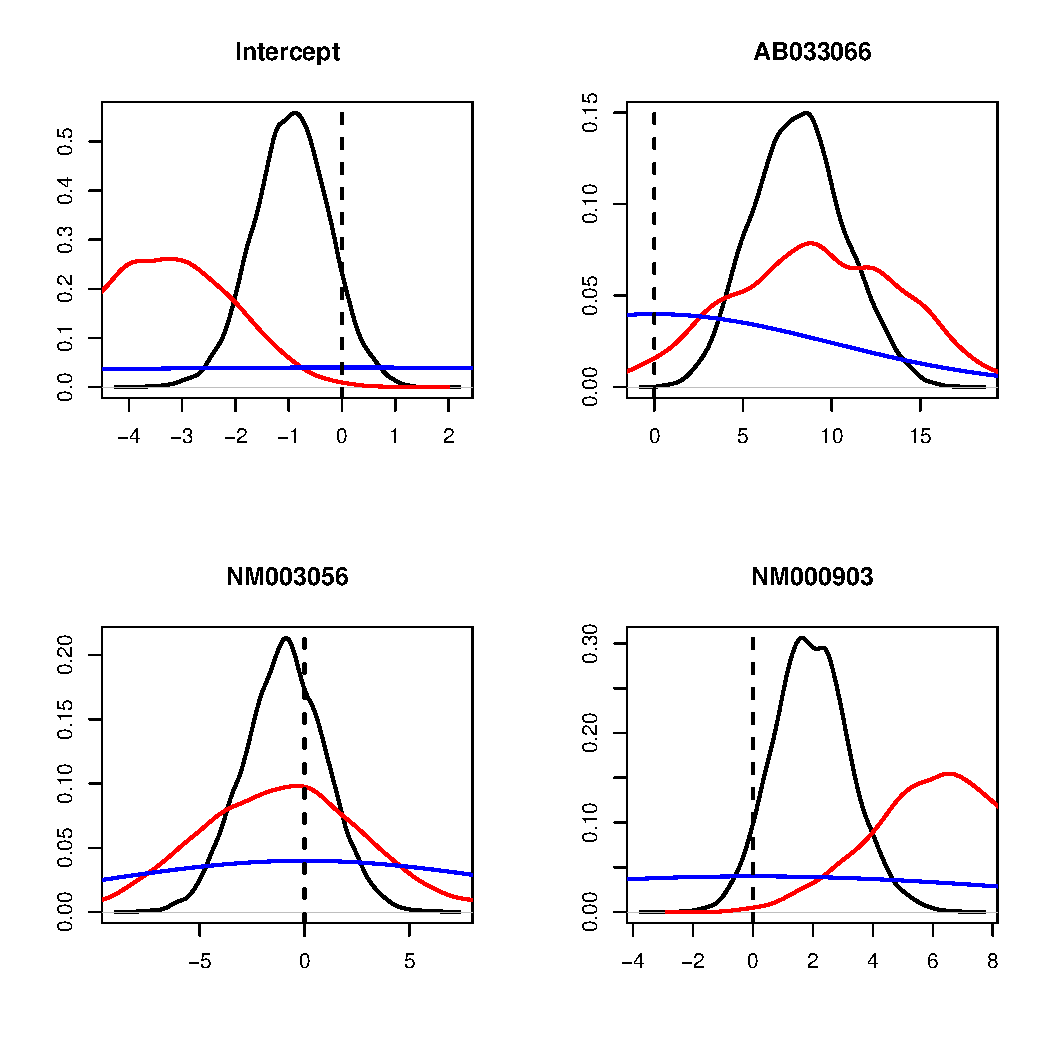
\includegraphics[width=.8\textwidth, height=.8\textheight]{\figfig/posterior-combine}
  $$
}

